\documentclass[a4paper,12pt]{article}

\usepackage[utf8]{inputenc}
\usepackage{amsfonts}
\usepackage{amssymb}
\usepackage{amsmath}
\usepackage{graphicx}
\title{\textbf{Introduction to Probability}}
\author{\textbf{Anche Kuo}}
\date{NCTU Computer Science}

\begin{document}
\maketitle

\begin{figure}[ht!]
\centering
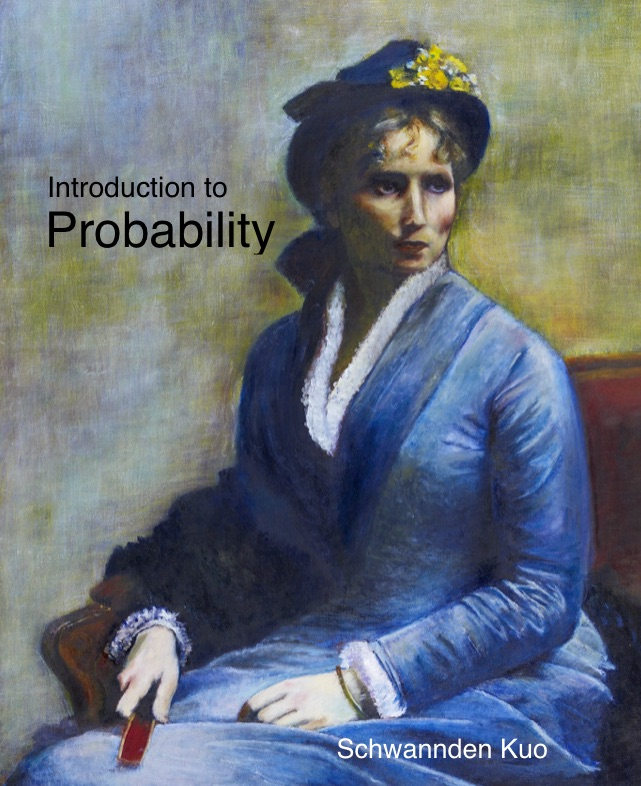
\includegraphics[width=90mm]{charlotteDubourg.jpg}

$$To\ my\ parent,\ Tiger\ and\ Sophie$$
$$Who\ gave\ me\ a\ world\ to\ dream\ and\ always\ encourage\ me\ to\ keep\ dreaming$$
\label{overflow}
\end{figure}

\newpage
\tableofcontents

\section{Statistical Inferences}

First recall the two definitions

\textbf{Definition}
Suppose we have a random variable with p.d.f $f(x, \theta)$ where $\theta$ is an unknown vector, we then call $\theta$ a parameter and the set of $\theta$'s possible values, denoted $\Theta$, is called the parameter space

\textbf{Definition}
For a random sample $X_1, ..., X_n$, any function $g(X_1, X_2, ..., X_n): $ independent of parameter $\theta$ is called a statistics.

Let $\mathbb{X} \sim f$ be a random variable, if we know p.d.f $f$, then we know everything we want with that random variable. The problem in statistics is that we have a random point from $\{ f(x, \theta) | \theta\in\Theta \}$ where function $f$ is known but parameter $\theta$ is unknown. Statistics wants to predict $\theta$. The method for predicting $\theta$ is called statistical inference. In the later text of this book, I shall refer "a random point from $\{ f(x, \theta) | \theta\in\Theta \}$" simply by "a random point from $f(x, \theta)$" for brevity.

Two kinds of statistical inference are called \textbf{estimation} and \textbf{hypothesis testing}. Estimation means we try to guess the value of $\theta$, hypothesis testing might not care about $\theta$, but test the the result of some experiment against the hypothesis. The key in hypothesis testing how sure can we know for certain, that the conclusion draw from the experiment is correct.

More formally, we categorize estimation into
(1) \textbf{Point estimate}: given $X_1, ..., X_n$, what is the function for estimating $\theta$ based solely on $X_1, ..., X_n$.
(2) \textbf{Interval estimate}: Given $\alpha\in[0, 1]$, find statistics $T_1(X_1, ..., X_n)$ and $T_2(X_1, ..., X_n)$ with $\alpha = \mathbb{P}_{\theta}( T_1 \leq \theta \leq T_2 )$

Point estimation is meaningless if we don't have interval estimation, because we need to be able to argue how good is the estimation. Put in other words, after point estimation gives us $\hat{\theta}$, we need interval estimation to tell us how close is this $\hat{\theta}$ compared to real $\theta$. That is what interval estimation does. Interval estimation introduces the notion of \textbf{confidence}. Confidence is the value $\alpha$ in (2). So interval estimation is, no matter how large is your confidence, we can tell you an interval such that the probability that $\theta$ lies within that interval is your confidence. This interval is called \textbf{confidence interval}. And of course, a good estimation has a smaller confidence interval for a given confidence.

And more formally, hypothesis testing is that given $\theta_0 \subset \mathbb{R}$ and hypothesis $H: \theta \in \theta_0$, find a rule to decide the acceptance of rejection of $H$. We will have more to say about interval estimation later.

\subsection{Point Estimate}

\textbf{Definition} We call a statistics $\hat{\theta} = \hat{\theta} (X_1, ..., X_n)$ an estimator of $\theta$ if it is used to estimate $\theta$. If $X_1 = x_1, ...,  X_n = x_n$ is observed, the value $\hat{\theta} (x_i, ..., x_n)$ is called estimate of $\theta$.

Two problems for point estimation:
(a) When many estimators are available, what is the criterion on "good" or "best" estimator.
(b) Need rules for deriving estimators, depending on the criterion. Two will be introduced.

Before we introduce the first criterion on a good estimator, let's recall the definition of expectation on multivariate random variable: 

If $T(X_1, ..., X_n)$ is a statistics (or an estimator), then
$$
\mathbb{E}[T(X_1, ..., X_n)] =
\begin{cases}
\int...\int T(x_1, ..., x_n)f(x_1, ..., x_n, \theta) \mathrm{d}x_1...\mathrm{d}x_2 & \text{for continnuous case.}
\sum...\sum T(x_1, ..., x_n)f(x_1, ..., x_n, \theta) & \text{ for discrete case.}
\end{cases}
$$

Now the first criterion is based on the expectation:

\textbf{Definition} We call an estimation \textbf{unbiased} for parameter $\theta$ if it satisfies
$\mathbb{E}_\theta [\hat{\theta}( X_1, ..., X_n )] = \theta$ for $\theta \in \Theta$.
Here $\mathbb{E}_\theta [\hat{\theta}( X_1, ..., X_n )]$ means we are taking expectation of $\hat{\theta}( X_1, ..., X_n )$ after $\theta$ is given.


\textbf{Example} $X_1, ..., X_n$ are i.i.d $normal( \mu, \sigma^2 )$. Our interest is $\theta = \mu$. $\mathbb{E}[X_1] = \mu$, so $\hat{\theta} = X_1$ is unbiased estimation of $\mu$. In fact, for all $k \in 1, 2, ..., n$, $\hat{\theta} = \frac{1}{k}\sum_{i_1 < i_2 < ...< i_k}X_i$ is unbiased estimation for $\mu$.

\textbf{Example} For $X \sim normal(0, \sigma^2)$, $X^2$ is an unbiased estimator for $X$'s variance, because $\mathbb{E}[X^2] = (\mathbb{E}[X])^2 + \sigma^2 = \sigma^2$

We want to seek the best estimator in the class of unbiased estimator, but what is best? Depending on the criterion, the best estimator might be different. One intuitive criterion would be, if we have enough points from a random sample, the estimate based on these sample points will be very close to the real point. This sounds like the notion of convergence in analysis, but in probability, how do you define "close to"? As the two point being compared with are functions(random variables).

In analysis, there is the notion of uniform convergence and point-wise convergence for sequence of functions, but both are too strict for probability. Two p.d.f's can be different on certain set of points but yield the same result under integration over identical set. That is, for p.d.f $f$ and $g$, it is possible that
$$f \neq g \text{ and } \forall_{A\subset \mathbb{R}} \int_A f = \int_A g$$

and that result of integration is all we want in probability, we want to know the probability of certain event. So in the field of probability, let's look at a weaker version of convergence, called convergence in probability.

\textbf{Definition} We say that $X_n$ converges to $X$ \textbf{in probability}, if for every $\epsilon > 0$, $\mathbb{P}(|X_n-X|>\epsilon) \to 0$ as $n \to \infty$. Denoted $X_n \overset{P}{\to} X$

With the notion of convergence in probability, let's look at the second criterion for a good estimator.

\textbf{Definition}  We call an estimation $\hat{\theta}$ \textbf{consistent} for $\theta$ if $\hat{\theta} \overset{P}{\to} \theta$

Here is a useful theorem to show if an estimator is consistent.

\textbf{Theorem} Suppose that the estimation $\hat{\theta} = \hat{\theta}(X_1, X_2, ..., X_n)$ of parameter $\theta$, satisfies $\mathbb{E}[\hat{\theta}] = \theta$ (unbiased), or $\mathbb{E}[\hat{\theta}] \to \theta$  (asymptotically unbiased) and
$var( \hat{\theta} ) \to 0$, then $\hat{\theta}$ is consistent for $\theta$, i.e,
$$\hat{\theta} \overset{P}{\to} \theta$$

Before proving this theorem, recall these two inequalities:
Marcov's inequality: if $X > 0$, then $\mathbb{P}(X\geq u) \leq \frac{\mathbb{E}[X]}{u}$
Chebyshev's inequality: If $\mathbb{E}[x] = \mu$ and $var(X) = \sigma^2$, then $\mathbb{P}(|X-\mu| \geq k\sigma) \leq \frac{1}{k^2}$

\textbf{Proof} $$\mathbb{E}[(\hat{\theta} - \theta)^2] = \mathbb{E}[(\hat{\theta} - \mathbb{E}[\hat{\theta}] + \mathbb{E}[\hat{\theta}] - \theta)^2]$$
$$= \mathbb{E}[(\hat{\theta} - \mathbb{E}[\hat{\theta}])^2] + 2\mathbb{E}[ (\hat{\theta} - \mathbb{E}[\hat{\theta}])(\mathbb{E}[\hat{\theta}] - \theta) ] + \mathbb{E}[(\mathbb{E}[\hat{\theta}] - \theta)^2]$$
$$=  \text{( } \mathbb{E}[\hat{\theta}] - \theta \text{ is contant with respect to } \hat{\theta} \text{ ) } var(\hat{\theta}) + 2\mathbb{E}[ \hat{\theta} - \mathbb{E}[\hat{\theta}]](\mathbb{E}[\hat{\theta}] - \theta) + (\hat{\theta} - \theta)^2$$
$$= \text{( } \mathbb{E}[ \hat{\theta} - \mathbb{E}[\hat{\theta}]] = 0 \text{ ) }var(\hat{\theta}) + (\mathbb{E}[\hat{\theta}] - \theta)^2$$
Finally by Marcov's inequality:
$$0 \leq \mathbb{P}( | \hat{\theta} - \theta | > \epsilon ) = \mathbb{P}( ( \hat{\theta} - \theta )^2 > \epsilon ) \leq \frac{\mathbb{E}[ ( \hat{\theta} - \theta )^2 ]}{\epsilon^2} \to 0$$

\textbf{Example} $\{X_n\}$ is a sequence of random variable, and
$$X_n \sim f_n(x) =
\begin{cases}
1-\frac{1}{2^n} & \text{if } x=0 
\frac{1}{2^n} & \text{if } x=1 
0 & \text{ otherwise }
\end{cases}$$
Show that $X_n \overset{P}{\to} 0$

\textbf{Solution} 

By definition:
Note for $\epsilon > 1$, $\mathbb{P}( |X_n - 0| > \epsilon ) = 0$ for all n, so we only look at $\epsilon\in(0, 1]$
$$\mathbb{P}( |X_n - 0| > \epsilon ) = \mathbb{P}( X_n = 1 ) = \frac{1}{2^n} \to 0$$

By theorem:
$\mathbb{E}[X_n] = \frac{1}{2^n} \to 0$ and $\mathbb{E}[X_n^2]-(\mathbb{E}[X_n])^2 = \frac{1}{2^n} - \frac{1}{2^{2n}} \to 0$, so by the above theorem, $X_n \overset{P}{\to} 0$

The following theorem offers a connection between consistency and unbiasedness.

\textbf{Theorem} Weak Law of Large Number( WLLN ).

If $X_1, ..., X_n$ is a random sample with finite mean $\mu$ and variance $\sigma^2$ exists, then $\bar{\mathbb{X}} \overset{P}{\to} \mu$

\textbf{Proof} Since $\mathbb{E}[\bar{\mathbb{X}}] = \mu$ and $var(\bar{\mathbb{X}}) = \frac{\sigma^2}{n} \to 0$, by the last theorem, $\bar{\mathbb{X}} \overset{P}{\to} \mu$.

Note how WLLN connects the axiomatic probability to the notion of relative frequency. This law basically tells you relative frequency will converge.

Recall that $var(\mathbb{X}) = \mathbb{E}[(\mathbb{X}-\mu)^2] = \mathbb{E}[\mathbb{X}^2] - \mathbb{E}[\mathbb{X}]^2$, so $ \mathbb{E}[\mathbb{X}^2] = var(\mathbb{X}) - \mathbb{E}[\mathbb{X}]^2$

\textbf{Example} $Y_1, ..., Y_n$ are i.i.d. $f(y) = 3y^2 I_{y\in[0,1]}$, show that there exists $a$ such that $\bar{Y} \overset{P} {\to} a$.
\textbf{Solution} Since $var(Y_i) = \frac{3}{5}-(\frac{3}{4})^2$ exists and $\mu = \frac{3}{4}$, by W.L.L.N, a = $\frac{3}{4}$

\textbf{Example} $Y_1, ..., Y_n \overset{i.i.d}{\sim} normal(\mu, \sigma^2), n=2k$. Show that estimator for variance $\hat{\sigma^2} = \frac{1}{2k}\sum_{i=1}^k(Y_{2i} - Y_{2i-1})^2$ is unbiased and consistent for $\sigma^2$.

\textbf{Solution}
$$Y_{2i} - Y_{2i-1} \sim normal(0, 2\sigma^2) \Rightarrow \frac{Y_{2i} - Y_{2i-1}}{\sqrt{2\sigma^2}} \sim normal(0, 1)$$
$$\Rightarrow\frac{\sum_{i=1}^k(Y_{2i} - Y_{2i-1})^2}{2\sigma^2} \sim \chi^2(k)$$
So
$$\mathbb{E}[ \hat{\sigma^2} ] = \mathbb{E}[\frac{\sigma^2}{k} \frac{\sum_{i=1}^k(Y_{2i} - Y_{2i-1})^2}{2\sigma^2}] = \sigma^2$$
and
$$var(\hat{\sigma^2}) = \frac{\sigma^4}{k^2} var(  \frac{\sum_{i=1}^k(Y_{2i} - Y_{2i-1})^2}{2\sigma^2} ) = \frac{2\sigma^4}{k} \to 0$$
So it is consistent and unbiased.

\textbf{Example} If $U_n \overset{\mathbb{P}}{\to} u, g(x)$ is continuous at $x=u$, show that $g(U_n) \overset{\mathbb{P}}{\to} g(u)$

\textbf{Solution} By continuity of $g$
$$\forall_{\epsilon > 0} \exists_{\delta>0} \forall_{x} |x-u|\leq\delta \to |g(x)-g(u)|\leq \epsilon$$
$$\Rightarrow \{ x\ : \ |g(x)-g(u)| > \epsilon \} \subset \{ x\ : \ |x-u|> \delta \}$$
So
$$\forall_{\epsilon > 0} \mathbb{P}( |g(x)-g(u)| > \epsilon ) \leq \mathbb{P}( |x-u|> \delta ) \to 0$$

\textbf{Example} $Y_1, ..., Y_n \overset{i.i.d}{\sim} f(y) = (\theta+1)y^\theta I_{\{y\in[0,1]\}}$, is $\frac{2\bar{Y}-1}{1-\bar{Y}} \overset{\mathbb{P}}{\to} \theta$?

\textbf{Solution} Let $g(x) = \frac{2x-1}{1-x}$, $g$ is continuous at $x = \frac{\theta+1}{\theta+2}$, so $$g(\bar{Y}) = \frac{2\bar{Y}-1}{1-\bar{Y}} \overset{\mathbb{P}}{\to} g(\frac{\theta+1}{\theta+2}) = \theta$$

\textbf{Definition} Moment: If $\mathbb{X}$ is a random variable having a p.d.f $f(x, \theta)$, its population kth moment is defined as
$$\mathbb{E}_\theta[X^k] = 
\begin{cases}
\sum_{\{x|f(x) > 0\}} x^k f(x, \theta) & \text{ if } \mathbb{X} \text{ is discrete }
\int_{-\infty}^\infty x^k f(x, \theta) \mathrm{d}x & \text{ if } \mathbb{X} \text{ is continuous }
\end{cases}$$

We estimate the population moment by sample kth moment as $$\frac{1}{n}\sum_{i=1}^n X_i^k$$
Why? Suppose that $X_1, ..., X_n$ is a random sample from $f(x, \theta)$. Then, $X_1^k, ..., X_n^k$ is a random sample, so each $X_i^k$'s has mean $\mathbb{E}_\theta[X_1^k]$ and variance $var_\theta( X_1^k )$

By, WLLN, if $X_1, ..., X_n$ is a random sample with mean $\mu$ and variance exists, then $\bar{\mathbb{X}} \overset{\mathbb{P}}{\to} \mu$. And since $X_1, ..., X_n$ is a random sample from $f(x, \theta)$, $\frac{1}{n}\sum_{i=1}^n X_i^k \overset{\mathbb{P}}{\to} \mathbb{E}_\theta[X^k]$

This following example shows why sample variance is called sample variance:

\textbf{Example} Let $X_1, ..., X_n$ be a random sample with mean $\mu$ and variance $\sigma^2$. The sample variance $S^2 = \frac{1}{n-1}\sum_{i=1}^n (X_i-\bar{X})^2$ is an unbiased ($\mathbb{E}[S^2] = \sigma^2$) and consistent ($S^2 \overset{\mathbb{P}}{\to} \sigma^2$) estimation for variance $\sigma^2$.

\textbf{Proof} 
$$\mathbb{E}[S^2] = \mathbb{E}[ \frac{1}{n-1}\sum_{i=1}^n (X_i-\bar{X})^2 ] = \frac{1}{n-1}\sum_{i=1}^n\mathbb{E}[ (X_i-\bar{X})^2 ]$$
$$= \frac{1}{n-1}\sum_{i=1}^n\mathbb{E}[ X_i^2-2X_i\bar{X}+\bar{X}^2 ] = \frac{1}{n-1}\sum_{i=1}^n\mathbb{E}[ X_i^2 ] -2\bar{X}\sum_{i=1}^n\mathbb{E}[X_i]+\sum_{i=1}^n\mathbb{E}[\bar{X}^2 ]$$
$$= \frac{1}{n-1}(\sum_{i=1}^n\mathbb{E}[ X_i^2] - n\mathbb{E}[\bar{X}^2]) = \frac{1}{n-1}(\sum_{i=1}^n (\sigma^2 + \mu^2) - n(\frac{\sigma^2}{n} + \mu^2) = \sigma^2$$
So $S^2$ is unbiased.
$$S^2 = \frac{1}{n-1}(\sum_{i=1}^n\mathbb{E}[ X_i^2] - n\mathbb{E}[\bar{X}^2]) = \frac{n}{n-1}(\frac{1}{n}\sum_{i=1}^n\mathbb{E}[ X_i^2] - \mathbb{E}[\bar{X}^2])$$
$$\overset{\mathbb{P}}{\to} \frac{n}{n-1} ( \mathbb{E}[\mathbb{X}^2] - \mathbb{E}[\bar{\mathbb{X}}^2] (\because \frac{1}{n}\sum_{i=1}^n\mathbb{E}[ X_i^2] \overset{\mathbb{P}}{\to} \mathbb{E}[\mathbb{X}^2]) = \sigma^2$$
So $S^2$ is consistent.

We now introduce two methods for estimation of $\theta$.

\subsubsection{Model of Moment}
Model of moment: Solve estimation from equations for estimating population moments by sample moments. This way it is guaranteed that the estimation will be unbiased for $\mathbb{E}[\mathbb{X}^k]$.

\textbf{Definition} Let $\mathbb{X}_1, ..., \mathbb{X}_n$ be a random sample from a distribution with p.d.f $f(x, \theta)$
(a) If $\theta$ is univariate, the method of moment estimator $\hat{\theta}$ solves $\theta$ for $$\bar{\mathbb{X}} = \mathbb{E}_\theta[\mathbb{X}]$$
(b) If $\theta = (\theta_1, \theta_2)$ is bivariate, the method of moment estimator $\hat{\theta} = (\hat{\theta_1}, \hat{\theta_2})$ solves
$$\begin{cases}
\bar{\mathbb{X}} = \mathbb{E}_{\theta_1, \theta_2}(\mathbb{X})
\frac{1}{n}\sum_{i=1}^n\mathbb{E}[ \mathbb{X}_i^2] = \mathbb{E}_{\theta_1, \theta_2}(\mathbb{X}^2)
\end{cases}
$$
(c) So in general, if $\theta = (\theta_1, ..., \theta_k)$ is k-variate, the method of moment estimator $\hat{\theta} = (\hat{\theta_1}, ..., \hat{\theta_k})$ solves
$$\begin{cases}
\frac{1}{n}\sum_{i=1}^n\mathbb{E}[ \mathbb{X}_i] = \mathbb{E}_{\theta_1, ...,  \theta_k}(\mathbb{X})
\frac{1}{n}\sum_{i=1}^n\mathbb{E}[ \mathbb{X}_i^2] = \mathbb{E}_{\theta_1, ..., \theta_k}(\mathbb{X}^2)
\vdots
\frac{1}{n}\sum_{i=1}^n\mathbb{E}[ \mathbb{X}_i^k] = \mathbb{E}_{\theta_1, ..., \theta_k}(\mathbb{X}^k)
\end{cases}$$

\textbf{Example} Suppose $X_1, ..., X_n \overset{i.i.d}{\sim} Bernoulli(p)$, we solve for
$$\frac{1}{n}\sum_{i=1}^n\mathbb{E}[ \mathbb{X}_i] = p \text{, so } \hat{p} = \bar{\mathbb{X}}$$
Note it is also consistent since $var(\bar{\mathbb{X}}) = \frac{p(1-p)}{n}\to 0$

\textbf{Example} Let $X_1, ..., X_n \overset{i.i.d}{\sim} Poisson(\lambda)$, find the method of moment estimation of $\lambda$, and see if it is unbiased and consistent.

\textbf{Solution} Solve
$$\bar{\mathbb{X}} = \mathbb{E}_\lambda[\mathbb{X}] \Rightarrow \hat{\lambda} = \bar{\mathbb{X}}$$
it is unbiased. And since
$$var(\hat{\lambda}) = var( \mathbb{\bar{X}} ) = \frac{\lambda}{n} \to 0$$ By WLLN, $\hat{\lambda} \overset{\mathbb{P}}{\to} \lambda$, so it is consistent.

Note if we want to find the method of moment estimation of $\theta = \sqrt{\lambda}$, just solve for $\hat{\lambda}$, then $\hat{\theta} = \sqrt{
\hat{\lambda}}$

\textbf{Example} Let $X_1, ..., X_n$ be a random sample, and each $X_i's$ has mean $\mu$ and variance $\sigma^2$. What is the method of moment estimation of $\theta = \{\mu, \sigma\}$

\textbf{Solution} Solve
$$\begin{cases}
\bar{\mathbb{X}} = \mu 
\frac{1}{n}\sum \mathbb{X}_i^2 = \mathbb{E}[\mathbb{X}^2] = \mu^2 + \sigma^2
\end{cases}$$
So $\hat{\mu} = \bar{\mathbb{X}}$, and $\hat{\sigma^2} = \frac{1}{n}\sum_{i=1}^n \mathbb{X}_i^2 - \hat{\mu}^2 = \frac{1}{n} (\sum_{i=1}^n \mathbb{X}_i^2 - n\bar{\mathbb{X}}^2)$. To prove that $\hat{\mu}$ is unbiased and consistent is trivial. But if we look at $\hat{\sigma^2}$ 
$$\mathbb{E}[\hat{\sigma^2}] = \mathbb{E}[ \frac{1}{n} \sum_{i=1}^n (\mathbb{X}_i^2 - \bar{\mathbb{X}}^2) ] = \frac{n-1}{n}\mathbb{E}[ \frac{1}{n-1} (\sum_{i=1}^n \mathbb{X}_i^2 - n\bar{\mathbb{X}}^2) ] = \frac{n-1}{n} \sigma^2$$
So $\hat{\sigma^2}$ is biased. But
$$\hat{\sigma^2} = \frac{1}{n} \sum (\mathbb{X}_i^2 - n\bar{\mathbb{X}}^2) \overset{\mathbb{P}}{\to} \mathbb{E}[\mathbb{X}^2] - \mu^2 = \sigma^2$$ Therefore, $\hat{\sigma^2}$ is consistent.

\subsubsection{Maximum Likelihood Estimation}

Let $X_1, ..., X_n$ be a random sample from $f(x, \theta), \theta \in \Theta$. The joint p.d.f $f(x_1, ..., x_n, \theta) = \prod_{i=1}^n f(x_i, \theta)$ for some $\theta \in \Theta$. As p.d.f, it satisfies
$$\forall_{\theta \in \Theta }\int_{-\infty}^\infty ... \int_{-\infty}^\infty f(x_1, ..., x_n, \theta) \mathrm{d}x_1 ... \mathrm{d}x_n = 1$$
\textbf{Definition} Given $x_1, ..., x_n$, the likelihood function of a random sample is defined on its joint p.d.f as a function of $\theta$
$$L(\theta) = f(x_1, ..., x_n, \theta), \theta \in \Theta$$

For $x_1, ..., x_n$ fixed, the value $L(\theta)$ is called the likelihood at $\theta$. We know that true $\theta$ is in the parameter space $\Theta$, but it is to be estimated from $X_1 = x_1, ..., X_n = x_n$.

If $L(\theta_1) > L(\theta_2)$, we consider that $\theta_1$ is more reliable than $\theta_2$ to be the true $\theta$ when $x_1, ..., x_n$ are given.

\textbf{Definition} When $X_1 = x_1, ..., X_n = x_n$ is observed, we have $L(\theta)$ corresponding to these $x_i's$. Let $\hat{\theta} = \hat{\theta}(X_1, ..., X_n)$ be any value of $\theta$ that maximizes $L(\theta)$, we then call $\hat{\theta}$ the maximum likelihood estimator(m.l.e) of $\theta$. When $X_1 = x_1, ..., X_n = x_n$ is observed, we call $\hat{\theta}(x_1, ..., x_n)$ the maximum likelihood estimate of $\theta$.

\textbf{Order statistics}
Let $X_1, ..., X_n$ be a random sample from from a distribution with p.d.f $f$ and c.d.f $F$. If $Y_1, ..., Y_n$ is a permutation of $X_1, ..., X_n$ such that $Y_1 \leq Y_2 \leq ... \leq Y_n$, we call $(Y_1, ..., Y_n)$ the order statistics of $(X_1, ..., X_n)$.

Some properties:
(a) $F_{Y_n}(y) = \mathbb{P}( Y_n \leq y ) = \mathbb{P}(X_1 \leq y, ..., X_n \leq y) = \prod_{i=1}^n \mathbb{P}(X_i \leq y) = F(y)^n$
(b) From (a), $f_{Y_n} (y) = n F(y)^{n-1}f(y)$
(c) $F_{Y_1}(y) = \mathbb{P}( Y_1 \leq y ) = 1-\mathbb{P}( Y_1 > y ) = 1-\mathbb{P}(X_1 > y, ..., X_n > y) = 1-\prod_{i=1}^n \mathbb{P}(X_i > y) = 1-(1-F(y))^n$
(d) From (c), $f_{Y_1} = n(1-F(y))^{n-1}f(y)$
(e) $f_{Y_i}(y) = {n \choose i-1, 1, n-i} F(y)^{i-1}f(y)(1-F(y))^{n-i}$

\textbf{Example} Let $X_1, ..., X_n \overset{i.i.d}{\sim} uniform(0, \theta)$, what is the m.l.e of $\theta$? Is this m.l.e unbiased or consistent?

\textbf{Solution} P.d.f of $X_i's$ is $f(x) = \frac{1}{\theta} I_{[0, \theta]}$

The likelihood function of $X_1, ..., X_n$, $L(\theta) = \prod_{i=1}^n \frac{1}{\theta} I_{X_i \in [0, \theta]} \neq 0$ if and only if $\forall_{i\in 1, ..., n} X_i \in [0, \theta]$. Let $Y_n = max(X_1, ..., X_n)$, then $L(\theta) = \frac{1}{\theta^n}I_{Y_n \in [0, \theta]}$. And the maximum of $L(\theta)$ is achieved at $\theta = max(x_1, ..., x_n)$.

The c.d.f of $X$ is
$$F(x) = \int_0^x \frac{1}{\theta}\mathrm{d}t = \frac{x}{\theta}, x\in [0, \theta]$$
The p.d.f of $\hat{\theta} = Y_n$ is
$$g_n(y) = n\frac{y^{n-1}}{\theta^n}, y \in [0, \theta]$$
so
$$\mathbb{E}[ \hat{\theta} ] = \mathbb{E}[Y_n] = \int_0^\theta y g_n(y) \mathrm{d}y = \int_0^\theta n\frac{y^n}{\theta^n} \mathrm{d}y = \frac{n}{n+1}\theta$$
$\Rightarrow$ m.l.e is not unbiased.

But
$\lim_{n\to\infty} \mathbb{E}[\hat{\theta}] \to 0$, so $\hat{\theta}$ is asymptotically unbiased. $\mathbb{E}[\hat{\theta}^2] = \mathbb{E}[y_n^2] = \frac{n}{n+2}\theta^2$, so
$$var(\hat{\theta}) = \frac{n}{n+2}\theta^2 - (\frac{n}{n+1}\theta)^2  \to 0 \Rightarrow \hat{\theta}\text{ is consistent for } \theta$$
Note that $\hat{\theta}' = \frac{n+1}{n}\hat{\theta}$ is unbiased and consistent (Think about it, it is actually very reasonable and intuitive that $\hat{\theta}'$ is a better estimator).

\textbf{Example} Let $Y \sim binomial(n, p)$, discuss m.l.e of p.

\textbf{Solution} Likelihood function of $Y$ given $Y=y $ is
$$L(p) = f_Y(y) = {n \choose y}p^y(1-p)^{n-y}$$
To find its maximum value, 
$$\mathrm{D}_p \ln( L(y, p) ) = \frac{y}{p} - \frac{n-y}{1-p} = 0 \text{ iff } p = \frac{y}{n}$$
So the m.l.e $\hat{p} = \frac{Y}{n}$. $\mathbb{E}[\hat{p}] = \frac{np}{n} = p$, so $\hat{p}$ is unbiased. 
And $var(\hat{p}) = var(\frac{Y}{n}) = \frac{1}{n^2}var(Y) = \frac{p(1-p)}{n} \to 0$, so $\hat{p}$ is consistent.

\textbf{Example} Let $X_1, ..., X_n \sim normal(\mu, \sigma^2)$, what is m.l.e of $\mu, \sigma^2$?

\textbf{Solution} The likelihood function $$L(\mu, \sigma^2) = \prod_{i=1}^n \frac{1}{\sqrt{2\pi \sigma^2}}e^{-\frac{(x_i-\mu)^2}{2\sigma^2}}$$
To find maximum value of $\mu$
$$\mathrm{D}_\mu \ln( L(\mu, \sigma^2) ) =  \mathrm{D}_\mu [\sum_{i=1}^n (-\frac{1}{2}\ln(2\pi\sigma^2) - \frac{(x_i-\mu)^2}{2\sigma^2} )] = \frac{(\sum_{i=1}^n x_i-n\mu)}{\sigma^2}$$
$$= 0 \text{ iff } \mu = \bar{x}, \text{ so } \hat{\mu} = \bar{X}$$
To find maximum value of $\sigma^2$
$$D_{\sigma^2} L(\bar{x}, \sigma^2) = -\frac{n}{\sigma} + \frac{\sum_{i=1}^n(x_i - \bar{x})^2}{\sigma^3} = 0 \text{ iff } \sigma^2 = \frac{\sum_{i=1}^n(x_i - \bar{x})^2}{n}$$
So $\hat{\sigma^2} = \frac{\sum_{i=1}^n(X_i - \bar{X})^2}{n}$.

$\hat{\mu}$ is unbiased and consistent is trivial. So we look only at $\sigma^2$.
$$\mathbb{E}[\hat{\sigma^2}] = \frac{\sigma^2}{n}\mathbb{E}[\frac{\sum_{i=1}^n(X_i - \bar{X})^2}{\sigma^2}] = \frac{n-1}{n} \sigma^2$$
Here we used the property $\frac{\sum_{i=1}^n(X_i - \bar{X})^2}{\sigma^2} \sim \chi^2(n-1)$. So $\hat{\sigma^2}$ is only asymptotically unbiased.
$$var(\hat{\sigma^2}) = \frac{\sigma^4}{n^2} var( \frac{\sum_{i=1}^n(X_i - \bar{X})^2}{\sigma^2} ) = \frac{\sigma^4}{n^2}2(n-1) \to 0$$
So $\hat{\sigma^2}$ is consistent.

\textbf{Example} $X_1, ..., X_n \overset{i.i.d}{\sim} uniform(0, 2\theta)$, find m.l.e of $\theta$.

\textbf{Solution} The likelihood function $L(\theta) = \prod_{i=1}^n \frac{1}{2\theta}I_{x_i\in[0, 2\theta]}(x_i) = \frac{1}{(2\theta)^n}I_{\theta\in\ [\frac{y_n}{2}, \infty]}(\theta)$. So $\hat{\theta} = \frac{Y_n}{2}$. Note that $\mathbb{E}[\frac{Y_n}{2\theta}] = \mathbb{E}[ beta(n, 1) ] = \frac{n}{n+1}$, so $\mathbb{E}[\frac{Y_n}{2}] = \frac{n\theta}{n+1}$.

\textbf{Example}  $X_1, ..., X_n \overset{i.i.d}{\sim} uniform(\theta_1, \theta_2), \theta_1 < \theta_2$, find m.l.e of $\theta_1, \theta_2$.

\textbf{Solution} The likelihood function $f(x, \theta) = \prod_{i=1}^n \frac{1}{\theta_2 - \theta_1}I_{x_i\in[\theta_1, \theta_2]}(x_i) = \frac{1}{(\theta_2 - \theta_1)^n}I_{\theta_1\in[-\infty, Y_1]}(\theta_1)I_{\theta_2\in[Y_n, \theta_2]}(\theta_2) $, so $\hat{\theta_1} = Y_1, \hat{\theta_n} = Y_n$
$$\mathbb{E}[Y_1] = \int_{\theta_1}^{\theta_2} n(1-\frac{y-\theta_1}{\theta_2-\theta_1})^{n-1}\frac{1}{\theta_2-\theta_1}y \mathrm{d}y = \frac{n}{(\theta_2-\theta_1)^n}\int_{\theta_1}^{\theta_2} (\theta_2-y)^{n-1}y\mathrm{d}y$$
$$= \frac{n}{(\theta_2-\theta_1)^n}( y[-\frac{(\theta_2-y)^n}{n}]_{\theta_1}^{\theta_2} + \int_{\theta_1}^{\theta_2}\frac{(\theta_2-y)^n}{n}\mathrm{d}y) = \frac{n\theta_1+\theta_2}{n+1}\to\theta_1$$
$$\mathbb{E}[Y_n] = \int_{\theta_1}^{\theta_2} n(\frac{y-\theta_1}{\theta_2-\theta_1})^{n-1}\frac{1}{\theta_2-\theta_1}y \mathrm{d}y = \frac{n}{(\theta_2-\theta_1)^n}\int_{\theta_1}^{\theta_2} (y-\theta_1)^{n-1}y\mathrm{d}y$$
$$= \frac{n}{(\theta_2-\theta_1)^n}( y[\frac{(y-\theta_1)^n}{n}]_{\theta_1}^{\theta_2} - \int_{\theta_1}^{\theta_2}\frac{(y-\theta_1)^n}{n}\mathrm{d}y) = \frac{\theta_1+n\theta_2}{n+1}\to\theta_2$$

\textbf{Example}$X_1, ..., X_n  $ are independent, and $X_i\sim poisson(\lambda x_i)$ find m.l.e of $\lambda$.

\textbf{Solution} The likelihood function $L$ given $X_1 = k_1, ..., X_n = k_n$ is observed, is $L(\lambda) = \prod_{i=1}^n e^{-\lambda x_i}\frac{(\lambda x_i)^{k_i}}{k_i!}$, so 
$$\frac{\mathrm{d}}{\mathrm{d}\lambda}\ln(L(\lambda)) = \frac{\mathrm{d}}{\mathrm{d}\lambda}\sum_{i=1}^n (k_i\ln(x_i\lambda)-x_i\lambda-\ln(k_i!)) = \sum_{i=1}^n(\frac{k_i}{\lambda}-x_i)$$ and $\frac{\mathrm{d}}{\mathrm{d}\lambda}\ln(L(\lambda)) = 0$ only when $\lambda = \frac{\sum k_i}{\sum x_i}$, and by second derivative test, we know this is when $L(\lambda)$ achieves maximum. So $\hat{\lambda} = \frac{\bar{Y}}{\bar{x}}$

\textbf{Example} $X_1, ..., X_n \overset{i.i.d}{\sim} Bernoulli(\theta), \Theta \in [0, \frac{1}{2}]$. Find m.l.e of $\theta$.

\textbf{Solution} The maximum likelihood function $L$ given $X_1 = x_1, ..., X_n = x_n$ is observed, is $L(\lambda) = \theta^{\sum x_i} (1-\theta)^{n-\sum x_i}$, and $\ln(L(\theta)) = \sum x_i \ln(\theta) + (n-\sum x_i)\ln(1-\theta)$
$$\frac{\mathrm{d}}{\mathrm{d}\lambda}\ln(L(\lambda)) = \frac{\sum x_i}{\theta} - \frac{(n-\sum x_i)}{1-\theta} = 0 \text{ if } \theta = \frac{\sum x_i}{n}$$
, and by second derivative test, we know this is when $L(\lambda)$ achieves maximum. Adding the restriction such that $\Theta \in [0, \frac{1}{2}]$, applying some simple calculus, we can show $\hat{\lambda} = min( \frac{1}{2}, \bar{X} )$


Suppose that we have $\hat{\theta} = \hat{\theta}(X_1, ..., X_n)$ for parameter $\theta$, and our intent is m.l.e of $\tau(\theta)$, a function of $\theta$. What is the m.l.e of $\tau(\theta)$?

The space of $\tau(\theta)$ is $\mathcal{T} = \tau(\Theta) = \{ z | \exists_{\theta\in\Theta}\ s.t\ \tau(\theta) = z\}$.

\textbf{Theorem} If $\hat{\theta} = \hat{\theta}(X_1, ..., X_n)$ is the m.l.e of $\theta$ and $\tau$ is a 1-1 function of $\theta$, then the m.l.e of $\tau(\theta)$ is $\tau(\hat{\theta})$

\textbf{Proof} Because $\tau$ is 1-1, for each $y\in\tau(\Theta)$, there exists a unique $x\in\Theta$ such that
$$L_{\tau(\theta)}(y) = L_{\theta}(x)$$
Where $L_{\tau(\theta)}$ and $L_{\theta}$ are likelihood function for $\tau(\theta)$ and $\theta$ respectively. And also
$$L_{\theta}(x) = L_{\theta}(\tau^{-1}(\tau(x)))$$
So $L_{\tau(\theta)} =  L_{\theta}(\tau^{-1})$. Now for all $t\in\tau(\Theta)$, we have
$$L_{\tau(\theta)}(y) =  L_{\theta}(\tau^{-1}(y)) = L_{\theta}(x) \leq L_{\theta}(\hat{\theta}) = L_{\tau(\theta)}(\tau(\hat{\theta}))$$

\textbf{Example} $Y \sim binomial(n, p)$, m.l.e of $p$ is $\hat{p} = \frac{Y}{n}$.
(1)$\sqrt{\frac{Y}{n}}$ is the m.l.e for $\tau = \sqrt{p}$
(2)$(\frac{Y}{n})^2$ is the m.l.e for $\tau = p^2$
(3)$e^{\frac{Y}{n}}$ is the m.l.e for $\tau = e^p$
(4)$\ln(\frac{Y}{n})$ is the m.l.e for $\tau = \ln(p)$

\subsubsection{Best Estimator: UMVUE}

An unbiased estimation $\hat{\theta} = \hat{\theta}( X_1, ..., X_n )$ is called a uniformly minimum variance unbiased estimation (UMVUE), or best estimation if for any unbiased estimator $\hat{\theta_i}$, we have
$$var_\theta(\hat{\theta}) \leq var_\theta(\hat{\theta_i}) \text{ for every } \theta \in \Theta$$
Two ways in deriving UMVUE will be introduced.

\textbf{Cramer-Rao lower bound } for UMVUE

Regularity conditions:
(a) Support of $X$ ( $\{ x | f(x, \theta) > 0 \}$ ) is an open interval
(b) Set $\{ x | f(x, \theta) = 0 \}$ or $\{ x | f(x, \theta) > 0 \}$ (support of f) is independent of $\theta$
(c)$\int \mathrm{D}_\theta f(x, \theta) \mathrm{d}x = \mathrm{D}_\theta \int f(x, \theta) \mathrm{d}x = 0$
(d)If $T = t(X_1, ..., X_n)$ is unbiased, then
$$\int ... \int t(x_1, .., x_n) \mathrm{D}_\theta f(x_1, ..., x_n, \theta) \mathrm{d}x_1...\mathrm{d}x_n = \mathrm{D}_\theta  \int ... \int t(x_1, .., x_n) f(x_1, ..., x_n, \theta) \mathrm{d}x_1...\mathrm{d}x_n $$ 

Some clarification here first, in (b), since p.d.f $f$ is positive, so $ \mathbb{R} = \{ x | f(x, \theta) = 0 \} \cup \{ x | f(x, \theta) > 0 \}$. This means either one of $\{ x | f(x, \theta) = 0 \}$ or $\{ x | f(x, \theta) > 0 \}$is independent of $\theta$.
 guarantees the independence of the other. In (c), on what condition is this allowed is given in appendix. 
 
\textbf{Theorem} (Cramer-Rao lower bound) Let $X_1, ..., X_n$ be a random sample from $f(x, \theta)$. Suppose that the regularity conditions hold. If $\hat{\tau}(\theta) = t(X_1, ..., X_n)$ is an unbiased estimator for $\tau(\theta)$, then
$$var_\theta(\hat{\tau}(\theta)) \geq \frac{(\tau'(\theta))^2}{n\mathbb{E}_\theta
[(\mathrm{D}_\theta \ln f(X_1, \theta))^2]} = \frac{(\tau'(\theta))^2}{-n\mathbb{E}_\theta
[\mathrm{D}_\theta^2 \ln f(X_1, \theta)]} \text{ for } \theta\in\Theta$$
\textbf{Proof} To simplify notation, we let $\textbf{X}$ be the random vector $(X_1, ..., X_n)$ and $\textbf{x} \in \mathbb{R}^n$ be a real vector. And we use $\Delta(\textbf{x},\theta)$ to denote $\prod_{i=1}^n f(x_1, \theta)$ . Now consider only the continuous distribution. First note that
$$E[\mathrm{D}_\theta \ln(f(X_1, \theta))] = \int_{-\infty}^\infty \mathrm{D}_\theta \ln{f(x, \theta)}\ f(x, \theta) \mathrm{d}x = \int_{-\infty}^\infty \mathrm{D}_\theta f(x, \theta) \mathrm{d}x = \mathrm{D}_\theta \int_{-\infty}^\infty f(x, \theta) \mathrm{d}x = 0$$
and $$\mathrm{D}_\theta \int ... \int \Delta(\textbf{x},\theta) \mathrm{d}x_1...\mathrm{d}x_n = \mathrm{D}_\theta 1 = 0$$
Since $\hat{\tau}(\theta)$ is unbiased
$$\tau(\theta) = \mathbb{E}_\theta[\hat{\tau}(\theta)] = \int ... \int t(\textbf{x}) \Delta(\textbf{x},\theta) \mathrm{d}x_1...\mathrm{d}x_n$$
Taking derivative on both sides, we have
$$\tau'(\theta) = \mathrm{D}_\theta \int ... \int t(\textbf{x}) \Delta(\textbf{x},\theta) \mathrm{d}x_1...\mathrm{d}x_n - \tau(\theta)\mathrm{D}_\theta \int ... \int \Delta(\textbf{x},\theta) \mathrm{d}x_1...\mathrm{d}x_n$$
$$\int ... \int t(\textbf{x}) \mathrm{D}_\theta \Delta(\textbf{x},\theta) \mathrm{d}x_1...\mathrm{d}x_n - \int ... \int \tau(\theta) \mathrm{D}_\theta \Delta(\textbf{x},\theta) \mathrm{d}x_1...\mathrm{d}x_n$$
$$= \int ... \int (t(\textbf{x}) - \tau(\theta)) \mathrm{D}_\theta \Delta(\textbf{x},\theta) \mathrm{d}x_1...\mathrm{d}x_n$$
Note $$\mathrm{D}_\theta \Delta(\textbf{x},\theta) = \sum_{j=1}^n D_\theta f(x_j, \theta)\prod_{i\neq j}f(x_i, \theta) = \sum_{j=1}^n [D_\theta \ln f(x_j, \theta) f(x_j, \theta) \prod_{i\neq j}f(x_i, \theta)]$$
$$= \sum_{j=1}^n D_\theta \ln f(x_j, \theta) \Delta(\textbf{x},\theta)$$
We now have
$$\tau'(\theta) = \int ... \int (t(\textbf{x}) - \tau(\theta)) \sum_{j=1}^n D_\theta \ln(f(x_j, \theta)) \Delta(\textbf{x},\theta) \mathrm{d}x_1...\mathrm{d}x_n $$
$$= \mathbb{E}_\theta [(t(\textbf{X}) - \tau(\theta)) \sum_{j=1}^n D_\theta \ln(f(X_j, \theta)]$$
And by Cauchy-Swartz inequality of random variable
$$(E[XY])^2\leq\mathbb{E}[X^2]\mathbb{E}[Y^2]$$
We have
$$(\tau'(\theta))^2 \leq {\mathbb{E}[(t(X_1, ..., X_n)} - \tau(\theta))^2]\mathbb{E}[(\sum_{j=1}^n D_\theta \ln(f(X_j, \theta)))^2]$$
and
$$\mathbb{E}[(\sum_{j=1}^n D_\theta \ln(f(X_j, \theta)))^2] = \sum_{j=1}^n \mathbb{E}[(D_\theta \ln(f(X_j, \theta)))^2] + \sum_{i\neq j}\mathbb{E}[D_\theta \ln(f(X_i, \theta))D_\theta \ln(f(X_j, \theta))]$$
$$= \sum_{j=1}^n \mathbb{E}[(D_\theta \ln(f(X_j, \theta)))^2] = n\mathbb{E}[(D_\theta \ln(f(X_1, \theta)))^2]$$
Hence
$$var(\hat{\tau}) = \mathbb{E}[(t(X_1, ..., X_n) - \tau(\theta))^2] \geq \frac{(\hat{\tau}'(\theta))^2}{n\mathbb{E}_\theta
[\mathrm{D}_\theta \ln(f(X_1, \theta))^2]}$$

It remains to prove the final equality, and showing $\mathbb{E}[(\mathrm{D}_{\theta} \ln f(\textbf{x}, \theta))^2] = - \mathbb{E}[ \mathrm{D}^2_\theta \ln f(\textbf{x}, \theta) ]$ suffice. Because
$$E[\mathrm{D}_\theta \ln(f(X_1, \theta))] = \int \mathrm{D}_\theta \ln f(\textbf{x}, \theta) f(\textbf{x}, \theta) \mathrm{d}x= 0$$
we can differentiate both sides and obtain
$$\mathrm{D}_\theta \int \mathrm{D}_\theta \ln f(\textbf{x}, \theta) f(\textbf{x}, \theta) \mathrm{d}x$$
$$= \int \mathrm{D}^2_\theta \ln f(\textbf{x}, \theta) f(\textbf{x}, \theta) + \mathrm{D}_\theta \ln f(\textbf{x}, \theta) \mathrm{D}_\theta f(\textbf{x}, \theta) \mathrm{d}x$$
$$= \int \mathrm{D}^2_\theta \ln f(\textbf{x}, \theta) f(\textbf{x}, \theta) + (\mathrm{D}_\theta \ln f(\textbf{x}, \theta))^2 f(\textbf{x}, \theta) \mathrm{d}x$$
$$= \mathbb{E}[ \mathrm{D}^2_\theta \ln f(\textbf{x}, \theta) ] + \mathbb{E}[(\mathrm{D}_{\theta} \ln f(\textbf{x}, \theta))^2] = 0$$
And the proof is complete.

\textbf{Theorem} If there is an unbiased estimator $\hat{\tau}(\theta)$ with variance achieving Cramer-Rao lower bound, then $\hat{\tau}(\theta)$ is UMVUE of $\tau(\theta)$

\textbf{Proof} By last theorem

\textbf{Example} Let $X_1, ..., X_n \overset{i.i.d}{\sim} Poisson(\lambda)$

\textbf{Solution} P.d.f of $X_i's$ is $f(x, \lambda)$, and
$$D_\lambda^2 \ln(f(x, \lambda)) = -\frac{x}{\lambda^2} \Rightarrow \frac{1}{-n\mathbb{E}_\theta
[\mathrm{D}_\theta^2 \ln(f(x, \theta))]} = \frac{\lambda}{n}$$
Since $\hat{\lambda} = \bar{X}$ has variance $\frac{\lambda}{n}$, it is UMVUE.

\textbf{Example} Let $X_1, ..., X_n \overset{i.i.d}{\sim} Bernoulli(p)$

\textbf{Solution} 
$$D_p \ln(f(x, p)) = \frac{x}{p} - \frac{1-x}{1-p}$$
$$D_p^2 \ln(f(x, p)) = -\frac{x}{p^2} - \frac{1-x}{(1-p)^2}$$
$$\mathbb{E}[ D_p^2 \ln(f(x, p)) ] = -\frac{1}{p(1-p)}$$
so Cramer-Rao lower bound is $\frac{p(1-p)}{n}$. And again, m.l.e of $p$, $\bar{X}$ is UMVUE of p.

\newpage
\section{Continuous to Point Estimation: sufficiency for UMVUE}

\textbf{Sufficient statistics}
Let A and B be two events. The conditional probability of A given B is defined as
$$\mathbb{P}(A|B) = \frac{\mathbb{P}(A\cap B)}{\mathbb{P}(B)}$$
And we showed that $\mathbb{P}(x|B)$ is a probability function too.

In estimation of $\theta$, we have a random sample $X_1, ..., X_n$ from distribution $f(x, \theta)$. The information we have abour $\theta$ is contained in $X_1, ..., X_n$.

Let $U = U(X_1, ..., X_n)$ be a statistic having p.d.f $f_U(u, \theta)$. The conditional p.d.f of $X_1, ..., X_n$ given $U=u$ is
$$f( x_1, ..., x_n, \theta | u ) = 
\begin{cases}
\frac{f(x_1, ..., x_n, \theta)}{f_U(u, \theta)} & \text{ if } u(x_1, ..., x_n) = u 
\frac{0}{f_U(u, \theta)} = 0 & \text{ if } u(x_1, ..., x_n) \neq u
\end{cases}$$

If for any $U = u$, conditional p.d.f $f(x_1, ..., x_n, \theta | u)$ is unrelated to $\theta$, i.e. $\forall_u\forall_{\theta_1, \theta_2} f(x_1, ..., x_n, \theta_1 | u) = f(x_1, ..., x_n, \theta_2 | u)$, then the random sample $X_1, ..., X_n$ contains no more information about $\theta$ then $U=u$ is observed. This indicates that $U=u$ contains information about $\theta$ exactly the same amount as $X_1, ..., X_n$.

\textbf{Definition} Let $X_1, ..., X_n$ be a random sample from $f(x, \theta), \theta\in\Theta$. We call a statistic $U=u(x_1, ..., x_n)$ a sufficient statistic if, for any value $U=u$, the conditional p.d.f $f(x_1, ..., x_n, \theta | u)$ and its domain do not depend on $\theta$.

\textbf{Example} Let $U = (X_1, ..., X_n)$, then
$$f(x_1, ..., x_n, \theta | u = (\acute{x}_1, ..., \acute{x}_n)) = 
\begin{cases}
\frac{f(\acute{x}_1, ..., \acute{x}_n, \theta)}{f(\acute{x}_1, ..., \acute{x}_n, \theta)} = 1 & \text{ if } (x_1, ..., x_n) = (\acute{x}_1, ..., \acute{x}_n) 
\frac{0}{f(\acute{x}_1, ..., \acute{x}_n, \theta)} = 0 & \text{ if } (x_1, ..., x_n) \neq (\acute{x}_1, ..., \acute{x}_n)
\end{cases}
$$
which is independent of $\theta$, so random sample $(X_1, ..., X_n)$ is a sufficient statstics.

\textbf{Example} Let $X_1, ..., X_n$ be a random sample from $f(x, \theta), \theta\in\Theta$. Consider the order statistics $Y_1, ..., Y_n$. If $(Y_1, ..., Y_n) = (y_1, ..., y_n)$ is observed, sample $X_1, ..., X_n$ has equal chance in the set 
$$A = \{ (x_1, ..., x_n)\in\mathbb{R}^n | (y_1, ..., y_n) \text{ is a permutation of } (x_1, ..., x_n) \}$$
Then the condition p.d.f of $X_1, ..., X_n$ given $(Y_1, ..., Y_n) = (y_1, ..., y_n)$ is
$$\begin{cases}
\frac{1}{n!} & \text{ if } (x_1, ..., x_n) \in A 
0 & \text{ otherwise}
\end{cases}$$
which is independent of $\theta$. Hence $(Y_1, ..., Y_n)$ is a sufficient statistic.

Why sufficiency?

We want a statistic with dimension as small as possible and that contains information about $\theta$ with the same amount as $(X_1, ..., X_n)$.

\textbf{Definition} If $U = U(X_1, ..., X_n)$ is a sufficient statistic whose range has the smallest dimension, it is called the minimal sufficient statistic.

\textbf{Example} Let $X_1, ..., X_n$ be a random sample from $Bernoulli(p), {p\in[0,1]}$, the joint p.d.f of $X_1, ..., X_n$ is
$$f(x_1, ..., x_n, p) = p^{\sum x_i}(1-p)^{n-\sum x_i}$$
Consider the statistics $Y = \sum_{i=1}^n X_i$ which has binomial distribution. The conditional p.d.f of $X_1, ..., X_n$ given $Y=y$ is $$f(\textbf{x}, p | y) = 
\begin{cases}
\frac{p^y(1-p)^{n-y}}{{n \choose y}p^y(1-p)^{n-y}} = \frac{y!(n-y)!}{n!} & \text{ if } \sum_{i=1}^n x_i = y 
\frac{0}{{n \choose y}p^y(1-p)^{n-y}} = 0 & \text{ otherwise}
\end{cases}$$  

So $Y$ is sufficient statistics. Furthermore, $Y$ is minimal sufficient statistic, because 1 is the minial possible dimension.

\textbf{Example} Let $X_1, ..., X_n$ be a random sample from $U(0, \theta)$. Show that the $n$th-order statistic $Y_n = max(X_1, ..., X_n)$ is a minimal sufficient statistic.

\textbf{Solution} The joint p.d.f of $X_1, ..., X_n$ is
$$f(x_1, ..., x_n, \theta) = 
\begin{cases}
\frac{1}{\theta^n} & \text{ if } x_i's \in [0, \theta]
0 & \text{otherwise}
\end{cases}$$
And recall that the p.d.f. of $Y_n$ is $f_{Y_n}(y) = n(\frac{y}{\theta})^{n-1}\frac{1}{\theta}$ for $y\in[0,\theta]$. When $Y_n = y$ is given, all $x_i's$ satisfies $x_i \leq y$. The conditional p.d.f of $X_1, ..., X_n$ given $Y_n = y$ is
$$f(x_1, ..., x_n, \theta | y) = 
\begin{cases}
\frac{f(x_1, ..., x_n, \theta, Y_n = y)}{f_{Y_n}(y)} =
 \frac{\frac{1}{\theta^n}}{n(\frac{y}{\theta})^{n-1}\frac{1}{\theta}} = \frac{1}{ny^{n-1}} & \text{ if } x_i's \leq y
0 & \text{otherwise}
\end{cases}$$

So $Y_n$ is a minimal sufficient statistic.

Now we want an easy way to derive sufficient statistics.

\textbf{Theorem} \textbf{(Factorization theorem)} Let $X_1, ..., X_n$ be a random sample from $f(x, \theta)$. A statistic $U = U(X_1, ..., X_n)$ is sufficient for $\theta$ if and only if there exists functions $K_1, K_2 \geq 0$ such that the joint p.d.f of $X_1, ..., X_n$ may be formulated as $f(x_1, ..., x_n, \theta) = K_1(U(x_1, ..., x_n), \theta)K_2(x_1, ..., x_n)$

\textbf{Proof} ($\Rightarrow$) If $U$ is sufficient, then the conditional p.d.f of $X_1, ..., X_n$ given $U=\mu$ is
$$f( x_1, ..., x_n, \theta | u ) = 
\begin{cases}
\frac{f(x_1, ..., x_n, \theta)}{f_U(u, \theta)} & \text{ if } u(x_1, ..., x_n) = \mu 
\frac{0}{f_U(u, \theta)} = 0 & \text{ if } u(x_1, ..., x_n) \neq \mu
\end{cases}$$
is unrelated to $\theta$. so $K_1 = f_U(u, \theta), K_2 = f(x_1, ..., x_n, \theta | u)$.

($\Leftarrow$) Suppose that $f(x_1, ..., x_n, \theta) = K_1(u(x_1, ..., x_n), \theta)K_2(x_1, ..., x_n)$. Let $Y_1 = u(X_1, ..., X_n)$, and for $i \in 2, ..., n$,  $Y_i = u_i(X_1, ..., X_n)$ be a 1-1 transformation with inverse function $X_i = w_i(Y_1, ..., Y_n)$, and Jacobian
$$J = \begin{vmatrix}
\frac{\partial x_1}{\partial y_1} & \cdots & \frac{\partial x_1}{\partial y_n}
\vdots & \ddots & \vdots
\frac{\partial x_n}{\partial y_1} & \cdots & \frac{\partial x_n}{\partial y_n}
\end{vmatrix}$$
The joint p.d.f of $Y_1, ..., Y_n$ is
$$f_{Y_1, ..., Y_n}(y_1, ..., y_n, \theta) = f( w_1(y_1, ..., y_n), ..., w_n(y_1, ..., y_n), \theta )|J|$$
$$= K_1(y_1, \theta)K_2(w_1(y_1, ..., y_n), ..., w_n(y_1, ..., y_n) )|J|$$
The p.d.f of $U = Y_1$ is
$$f_U(y, \theta) = \int...\int K_1(y_1, \theta)K_2(w_1(y_1, ..., y_n), ..., w_n(y_1, ..., y_n) )|J|\mathrm{d}y_2...\mathrm{d}y_n$$
$$= K_1(y_1, \theta) \int...\int K_2(w_1(y_1, ..., y_n), ..., w_n(y_1, ..., y_n) )|J|\mathrm{d}y_2...\mathrm{d}y_n$$
And note that everything in the integral is unrelated to $\theta$. Then the conditional p.d.f of $X_1, ..., X_n$ given $U=u$ is
$$f(x_1, ..., x_n, \theta | u) = 
\begin{cases}
\frac{f(x_1, ..., x_n, \theta)}{f_U(u, \theta)} = \frac{K_2(x_1, ..., x_n)}{\int...\int K_2\mathrm{d}y_2...\mathrm{d}y_n} & \text{ if } u(x_1, ..., x_n) = u
0 & \text{ otherwise }
\end{cases}$$ 

\textbf{Example} $X_1, ..., X_n \overset{i.i.d}{\sim} Poisson(\lambda)$, so joint p.d.f of $X_1, ..., X_n$ is
$$f(x_1, ..., x_n, \lambda) = \prod_{i=1}^n \frac{\lambda^{x_i} e^{-\lambda}}{x_i!}$$
$(X_1, ..., X_n), \sum X_i, \bar{X}$ are all sufficient.

\textbf{Example} $X_1, ..., X_n \overset{i.i.d}{\sim} normal(\mu, \sigma^2)$, want sufficient statistic from $(\mu, \sigma^2)$.

\textbf{Solution} Joint p.d.f of $X_1, ..., X_n, \mu, \sigma^2$ is
$$\prod_{i=1}^n \frac{1}{\sqrt{2\pi\sigma}}e^{-\frac{(x_i-\mu)^2}{2\sigma^2}} = (2\pi)^{-\frac{n}{2}}(\sigma^2)^{-\frac{n}{2}}e^{-\frac{\sum(x_i-\mu)^2}{2\sigma^2}}$$

$$\sum(x_i-\mu)^2 = \sum(x_i-\bar{x}+\bar{x}-\mu)^2 = \sum(x_1-\bar{x})^2 + n(\bar{x}-\mu)^2+2(\bar{x}-\mu)\sum(x_i-\bar{x})$$
$$(n-1)S^2+n(\bar{x}-\mu)^2$$

$$\Rightarrow f(x_1, ..., x_n, \mu, \sigma^2 ) = (2\pi)^{-\frac{n}{2}}(\sigma^2)^{-\frac{n}{2}}e^{-\frac{(n-1)S^2+n(\bar{x}-\mu)^2}{2\sigma^2}} * 1$$
$\Rightarrow (\bar{X}, S^2) $ is minimal sufficient for $ (\mu, \sigma^2) $

\textbf{Definition} $(X, Y)$ are random variables, conditional mean of $\mathbb{Y}$ given $X=x$, $\mathbb{E}[Y|X]$ is defined as
$$\int yf(y|x) \mathrm{d}y$$
Conditional variance of $\mathbb{Y}$ given $X=x$, $var(Y|X)$ is defined as
$$\mathbb{E}[ (Y - \mathbb{E}[Y|X])^2 |X ] = \int (y-\mathbb{E}[Y|X])^2 f(y|x) \mathrm{d}y = 
\mathbb{E}[ Y^2 |X ] - (\mathbb{E}[Y|X])^2$$

Note both conditional mean and condition variance of $Y$ given $X=x$ are actually function of x. So here we distinguish the constant value of conditional mean (when $x$ is given) and the its general form

\textbf{Definition} random conditional mean is $\mathbb{E}[Y|X]$ and random variance is $var(Y|X)$.

\textbf{Theorem}
(a)$\mathbb{E}[\mathbb{E}[Y|X]] = \mathbb{E}[Y]$
(b)$var(Y) = \mathbb{E}[var(Y|X)]+var(\mathbb{E}[Y|X])$

\textbf{Proof}
(a) trivial
(b) $var(Y|X) = \mathbb{E}[ Y^2 |X ] - (\mathbb{E}[Y|X])^2$, so $\mathbb{E}[var(Y|X)] = \mathbb{E}[Y^2] - \mathbb{E}[(\mathbb{E}[Y|X])^2]$. And $var(\mathbb{E}[Y|X]) = \mathbb{E}[ \mathbb{E}[Y|X]^2 ] - (\mathbb{E}[\mathbb{E}[Y|X]])^2 = \mathbb{E}[Y]^2$. Therefore $\mathbb{E}[var(Y|X)]+var(\mathbb{E}[Y|X]) = \mathbb{E}[ Y^2 |X ] - \mathbb{E}[Y]^2$

\textbf{Theorem} (Rao-blackwell) If $\hat{\tau}(X_1, ..., X_n)$ is an unbiased estimation of $\tau(\theta)$ and $U = U(X_1, ..., X_n)$ is sufficient for $\theta$, then
(a) $\mathbb{E}[ \hat{\tau}(X_1, ..., X_n) | U ]$ is a statistic
(b) $\mathbb{E}[ \hat{\tau}(X_1, ..., X_n) | U ]$ is unbiased for $\tau(\theta)$
(c) $var_\theta( \mathbb{E}[ \hat{\tau}(X_1, ..., X_n) | U ] )\leq var_\theta( \hat{\tau}(X_1, ..., X_n) )$ for $\theta\in\Theta$

\textbf{Proof}
(a) trivial, since the expection is integrating on terms unrelated to $\theta$
(b) $\mathbb{E}_\theta[ \mathbb{E}[ \hat{\tau}(X_1, ..., X_n) | U ] ] = \mathbb{E}[ \hat{\tau}(X_1, ..., X_n) ] = \tau(\theta)$
(c) $var_\theta( \hat{\tau}(X_1, ..., X_n) ) = \mathbb{E}_\theta[ var_\theta( \hat{\tau}(X_1, ..., X_n) | U) ] + var_\theta( \mathbb{E} [ \hat{\tau}(X_1, ..., X_n) | U ] )$
$$\Rightarrow var_\theta( \hat{\tau}(X_1, ..., X_n) ) \geq var_\theta( \mathbb{E} [ \hat{\tau}(X_1, ..., X_n) | U ] )$$

Rao-blackwell theorem gives us a way to improve on unbiased statistic, but we still need other idea to further understand the limitation of this improvement.

Let $U$ be a statistic. If $h(U) = 0$ or $\mathbb{P}(h(U)=0)=1$, then p.d.f of $h(U)$ is
$$f_{h(U)}(x) = 
\begin{cases}
1 & \text{ if } x=0
0 & \text{ otherwise }
\end{cases}$$
Then
$$\mathbb{E}_\theta[ h(U) ] = 0$$
That is, if $h(U) = 0$ or $\mathbb{P}(h(U)=0)=1$, then for all $\theta\in\Theta$, $\mathbb{E}_\theta[ h(U) ] = 0$.

However, for any $U$, if for all $\theta\in\Theta$, we have $\mathbb{E}_\theta[h(U)] = 0$, it is not necessary that $\mathbb{P}(h(U)=0)=1$.

\textbf{Example} Let $X_1, X_2 \overset{i.i.d}{\sim} normal(\mu, \theta)$. $U = X_1 - X_2$, and let $h(U) = U$. And we have $\mathbb{E}_{\mu, \sigma^2}[U] = 0$, but $\mathbb{P}(h(U)=0)=0$

\textbf{Definition} Let $X_1, ..., X_n$ be a random sample from $f(x, \theta)$, a statistic $U = U(X_1, ..., X_n)$ is a complete statistic if for any function $h$ such that $E_\theta[h(U)] = 0$, then
$$\mathbb{P}(h(U)=0)=1 \text{ for } \theta\in\Theta$$

To verify $\mathbb{P}( h(U) = 0 ) = 1$, it is sufficient to prove that $U(\mathbb{R}) - \{h(U) = 0\}$ has measure zero. Notice if $\{h(U) = 0\} \supset U(\mathbb{R})$, then $U(\mathbb{R}) - \{h(U) = 0\} = \emptyset$, and empty set has measure zero.

\textbf{Example} If $X_1, ..., .X_n \overset{i.i.d}{\sim} Bernoulli(p)$, we can show $Y = \sum X_i$ is complete. Suppose a function $h$ satisfies $\mathbb{E}( h(Y) = 0 ) = 1$ for all $p$, then
$$\sum_{k=0}^n h(k) {n \choose k} p^k(1-p)^{n-k} = (1-p)^n\sum_{k=0}^n h(k) {n \choose k} (\frac{p}{1-p})^k = 0 \text{ for all } p$$
But a polynomial with non-zero coefficient has at most k roots, so it must be the case that $h(k) {n \choose k} = 0 $ for $k = 0, 1, ..., n$. And this implies $h(k)= 0 $ for $k = 0, 1, ..., n$. So the range of $Y$ = $\{0, 1, ..., n \} \subset \{h(k)= 0\}$.

\textbf{Example} If $X_1, ..., .X_n \overset{i.i.d}{\sim} unifrom(\theta)$, we can show $Y_n = max(X_1, ..., X_n)$ is sufficient and complete.
1. We have shown $Y_n$ is sufficient by definition, now we do it by factorization. The joint p.d.f of $X_1, ..., X_n$ is
$$f(x_1, ..., x_n, \theta) = \prod_{i=1}^n \frac{1}{\theta^n} I_{\{Y_n \leq \theta\}} * 1$$
with $K_1 = f(x_1, ..., x_n, \theta), K_2 = 1$.
2. To show it is complete, for any function $h$, if for any $\theta\in\Theta$ we have
$$\mathbb{E}[ h(Y_n) ] = \int_0^\theta n\frac{y^{n-1}}{\theta^n}h(y) \mathrm{d}y = \frac{n}{\theta^n} \int_0^\theta y^{n-1}h(y) \mathrm{d}y = 0$$
So for all $\theta$, $\{ y | h(y) \neq 0 \}$ has measure zero in $[0, \theta]$, and so $\mathbb{P}( h(Y) = 0 ) = 1$

\textbf{Theorem} (Lehmann-Scheffe) Let $X_1, ..., X_n$ be a random sample from $f(x, \theta)$, suppose that $U = U(X_1, ..., X_n)$ is a complete and sufficient statistic. If $\hat{\tau}(\theta) = t(U)$ is an unbiased estimator for $\tau(\theta)$, then $\hat{\tau}(\theta)$ is the unique function of $U$ that is unbiased for $\tau(\theta)$ and is UMVUE of $\tau(\theta)$. Note we say two random random variables $X, Y$ are equal if $\mathbb{P}( X = Y ) = 1$ So here we say $\hat{\tau}(\theta)$ is the unique function of $U$ that is unbiased for $\tau(\theta)$, it means
$$\forall_{\text{ r.v } Y } \ Y \text{ is function of } U \text{ that is unbiased for } \tau(\theta) \to \mathbb{P}(Y = \hat{\tau}(\theta)) = 1$$

\textbf{Proof}
First I will prove function of $U$ that's unbiased is unique. Suppose $\acute{\tau}(\theta) = \acute{U}$ is also unbiased for $\tau(\theta)$, then
$$\mathbb{E}[ \hat{\tau}(\theta) - \acute{\tau}(\theta) ] = \mathbb{E}[ \hat{\tau}(\theta) ] - \mathbb{E}[ \acute{\tau}(\theta) ] = \tau(\theta) - \tau(\theta) = 0$$
And since $U$ is complete and $\hat{\tau}(\theta) - \acute{\tau}(\theta)$ is a function of $U$, we know 
$$\mathbb{P}( \hat{\tau}(\theta) - \acute{\tau}(\theta) = 0 ) = \mathbb{P}( \hat{\tau}(\theta) = \acute{\tau}(\theta) ) = 1$$

Second let's prove that it is UMVUE. If $T$ is any unbiased statistic for $\tau(\theta)$, then since $U$ is sufficient, Rao-Blackwell theorem, applies, and we have:
(1). $\mathbb{E}[ T | U ]$ is an unbiased statistics.
(2). $var( \mathbb{E}[ T | U ] ) \leq var( \mathbb{E}[ T ] )$

By first step and (1), $var( \mathbb{E}[ T | U ] )$ is an unique unbiased statistics, and (2) completes proof.


\pagebreak
In this class we will introduce confidence interval (CI), and hypothesis testing. Before this, we have to introduce a real distribution.

\textbf{Definition} (t-distribution) Suppose that we have
$$
\begin{cases}
\mathbb{Z} \sim \mathbb{N}(0, 1) 
\mathbb{V} \sim \mathbb{\chi}^2(r)
\end{cases}
$$
, and the two r.v are independent. We say that $\mathbb{T} = \frac{\mathbb{Z}}{\sqrt{\mathbb{V}/r}}$ has a t-distribution with d.f.r.

We also denote $\mathbb{T}\sim t(r)$.

\textbf{Theorem} If  $\mathbb{T}\sim t(r)$, its p.d.f is
$$f_\mathbb{T}(t) = \frac{\Gamma(\frac{r+1}{2})}{\sqrt{\pi r}\Gamma(\frac{r}{2})(1+\frac{t^2}{r})^\frac{r+1}{2}}, t\in\mathbb{R}$$

\textbf{Proof} Since $\mathbb{T}\sim t(r)$, $\mathbb{T} = \frac{\mathbb{Z}}{\sqrt{\mathbb{V}/r}}$. The joint p.d.f of $\mathbb{Z}$ and $\mathbb{V}$ is

$$f_{\mathbb{Z}\mathbb{V}}(\zeta, v) = 
\frac{1}{\sqrt{2\pi}} e^{-\frac{\zeta^2}{2}} \frac{1}{\Gamma(\frac{r}{2})2^{\frac{r}{2}}}v^{\frac{r}{2}-1}e^{-\frac{v}{2}}
, \zeta\in\mathbb{R}, v>0 $$

We consider transformation $\mathbb{T} = \frac{\mathbb{Z}}{\sqrt{\mathbb{V}/r}}$, $\mathbb{U} = \mathbb{V}$, we have
$$A = \big\{ {\zeta \choose v}: \zeta\in\mathbb{R}, v>0 \big\} \overset{{\mathbb{T} \choose \mathbb{U}}}{\to} B \big\{ {t \choose u}:t\in\mathbb{R}, u>0 \big\}$$

For ${t \choose u} \in B$, we have inverses $v=u, \zeta=\frac{\sqrt{u}t}{\sqrt{r}}$. Uniqie solution indicates 1-1 transformation. Jacobian is
$$J = 
\begin{vmatrix}
\frac{\partial \zeta}{\partial t} & \frac{\partial \zeta}{\partial u} 
\frac{\partial v}{\partial t} & \frac{\partial v}{\partial u}
\end{vmatrix} = 
\begin{vmatrix}
\frac{\sqrt{u}}{\sqrt{r}} & \frac{u^{-\frac{1}{2}}t}{2\sqrt{r}} 
0 & 1
\end{vmatrix}
= \frac{\sqrt{u}}{\sqrt{r}}$$

The joint p.d.f of $\mathbb{T}$ and $\mathbb{U}$ is
$$f_{\mathbb{T}\mathbb{U}} = f_{\mathbb{Z}\mathbb{V}}(\frac{\sqrt{u}t}{\sqrt{r}}, u)\frac{\sqrt{u}}{\sqrt{r}} = 
\frac{1}{\sqrt{2\pi}} e^{-\frac{1}{2}\frac{u}{r}t^2} \frac{1}{\Gamma(\frac{r}{2})2^{\frac{r}{2}}}u^{\frac{r}{2}-1}e^{-\frac{u}{2}}\frac{\sqrt{u}}{\sqrt{r}}$$

So

$$\mathbb{T} = \frac{1}{\sqrt{2\pi r}} \frac{1}{\Gamma(\frac{r}{2})2^{\frac{r}{2}}}
\int_0^\infty e^{-\frac{1}{2}(1+\frac{t^2}{r})u} u^{\frac{r+1}{2}-1}\mathrm{d}u$$
$$= \frac{1}{\sqrt{\pi r}\Gamma(\frac{r}{2})2^{\frac{r+1}{2}}} \frac{1}{(\frac{1}{2}(1+\frac{t^2}{r}))^{\frac{r+1}{2}}}
\int_0^\infty (\frac{1}{2}(1+\frac{t^2}{r}))^{\frac{r+1}{2}}e^{-\frac{1}{2}(1+\frac{t^2}{r})u} u^{\frac{r+1}{2}-1}\mathrm{d}u$$
$$= \frac{\Gamma(\frac{r+1}{2})}{\sqrt{\pi r}\Gamma(\frac{r}{2})(1+\frac{t^2}{r})^{\frac{r+1}{2}}}$$

Properties of $\mathbb{T}\sim t(r)$:
1. $ f_T(-t) = f_T(t)$, for $t>0 \Rightarrow f_T(t)$ is symmetric at $t=0$

The problem in statistics is that we have a random sample $X_1 ... X_n$ from $f(x, \theta)$, where $\theta$ is unknown parameter. The point estimate wants to know what is $\theta$ by defining estimation $\hat{\theta} = \hat{\theta}(X_1, ..., X_n)$. Although we can find unknown $\theta$on consistent estimation, or even UMVUE. However, if $\hat{\theta}(X_1, ..., X_n)$ has a continuous distribution, we have $\mathbb{P}_\theta(\hat{\theta}(X_1, ..., X_n) = \theta) = 0$ for $\theta \in \Theta$.

There is no confidence to claim that $\theta = \hat{\theta}$. We then want one approach that assume some confidence for $\theta$.

Confidence Interval

\textbf{Definition} Suppose we hae a random sample from $f(x, \theta)$. If there are two statistics $T_1 = t_1(X_1, ..., X_2)$ and 
$T_2 = t_2(X_1, ..., X_2)$ s.t
$$1-\alpha = \mathbb{P}_\theta(T_1 \leq \theta \leq T_2)$$
We call the random interval $(T_1, T_2)$ a $100(1-\alpha)\%$ confidence interval for $\theta$. We also call $(t_1(X_1, ..., X_2), t_2(X_1, ..., X_2))$ a $100(1-\alpha)\%$ CI interval for $\theta$.

Interpretation of C.I.:


(a) A $100(1-\alpha)\%$ C.I. $(T_1,T_2)$ means that it covers the unknown $\theta$ with probability $1-\alpha$. If we sample $X_1...X_n$ many times (m),
then the average $$\frac{1}{m} \sum_{j=1}^m I(t_1^{(j)} \leq \theta \leq t_2^{(j)}) \sim 1-\alpha$$.

(b) If $T_1 = t_1, T_2 = t_2$ is observed (once),
 then $\mathbb{P}_\theta (t_1 \leq \theta \leq t_2)$ is $0$ or $1$.

How to construct C.I.

\textbf{Definition} A function of random sample and parameter $\theta$,
 $ \mathbb{Q} = q( X_1...X_n, \theta)$ is called a pivotal quantity if its distribution is independent of $\mathbb{Q}$.
 
For each pivotal quantity $\mathbb{Q} = q( X_1...X_n, \theta)$, 
there are $a, b \in \mathbb{R}$ such that $$ 1-\alpha = \mathbb{P}_\theta (a \leq q( X_1... X_n, \theta) \leq b)$$ for $\theta \in \Theta$. Not all pivotal quantity can be used to construct C.I.
 
The interesting pivotal quantity is one which 1-1 transformation as:
 $$a \leq q(X_1 ... X_n, \theta) \leq b$$ if and only if $T_1 \leq \theta \leq T_2$ 
 for some statistics $T_1 = t_1 (X_1 ... X_n)$ and $T_2 = t_2 (X_1 ... X_n)$.

Hence, $1 -\alpha = \mathbb{P}_\theta (a \leq q(X_1 ... X_n, \theta) \leq b) = \mathbb{P}_\theta (T_1 \leq \theta \leq T_2)$ and $(T_1, T_2)$ is a $100(1-\alpha)\%$ C.I. for $\theta$.

Let $\mathbb{Z}$ be the r.v. with standard normal distribution $\mathbb{N}(0,1)$.
Denote $\zeta_\alpha$ with $\alpha = \mathbb{P}(\mathbb{Z} \geq \zeta_\alpha)$ 
or $1-\alpha = \mathbb{P}(\mathbb{Z} \leq \zeta_\alpha)$. 
We need $\zeta$ since it satisfies $1-\alpha = \mathbb{P}(-\zeta_{\frac{\alpha}{2}}\leq \mathbb{Z} \leq \zeta_{\frac{\alpha}{2}})$.

C.I. for normal mean.

Let $X_1 ... X_n$ be random samples from $\mathbb{N}(\mu,\sigma^2)$, 
want for $100(1-\alpha)\%$ C.I. for $\mu$. We consider two cases.

Case 1: $\sigma = \sigma_0$ is known.

We have $X_1 ... X_n \overset{i.i.d}{\sim} \mathbb{N}(\mu, \sigma^2)$ where $\sigma^2$ is known constant.
$$\bar{X} \sim \mathbb{N}(\mu, \frac{\sigma_0^2}{n}) \Rightarrow 
\bar{X} - \mu \sim \mathbb{N}(0, \frac{\sigma^2}{n}), 
\frac{(\bar{X} - \mu) \sqrt{n}}{\sigma_0} $$

$$\Rightarrow 1-\alpha = \mathbb{P}(-\zeta_{\frac{\alpha}{2}} \leq \mathbb{Z} \leq \zeta_{\frac{\alpha}{2}})
= \mathbb{P}(-\zeta_{\frac{\alpha}{2}} \leq \frac{(\bar{X} - \mu) \sqrt{n}}{\sigma_0} \leq \zeta_{\frac{\alpha}{2}})$$


$$= \mathbb{P} (-\zeta_{\frac{\alpha}{2}} \frac{\sigma_0}{\sqrt{n}} \leq \bar{X} - \mu \leq \zeta_{\frac{\alpha}{2}} \frac{\sigma_0}{\sqrt{n}}
= \mathbb{P}(\bar{X} - \zeta_{\frac{\alpha}{2}} \frac{\zeta_0}{\sqrt{n}}
\leq \mu \leq \bar{X} + \zeta_{\frac{\alpha}{2}} \frac{\sigma_0}{\sqrt{n}})$$

So C.I. for $\mu$ is $(\bar{X}- \zeta_{\frac{\alpha}{2}} \frac{\sigma_0}{\sqrt{n}},
\bar{X} + \zeta_{\frac{\alpha}{2}} \frac{\sigma_0}{\sqrt{n}})$



\newpage
\title{\textbf{{\LARGE Appendix}}}

Appendix provides proof to harder theorems. Some of which require background in analysis.


\paragraph{ A.1 \ \  Interchanging Differentiation and Integration}
If f(x, t) is a function of two variables, satisfying the following 3 conditions:
(1) f(x, t) exists on a closed cell $[a, b] \times [c, d]$
(2) $\forall_{t\in[c, d] }\ \ \int_a^b f(x, t) \mathrm{d}x$ exists
(3) Given $s \in (c, d)$, for any $\epsilon > 0$ corresponds a $\delta$ such that $$ | \mathrm{D}_2 f(x, t) - \mathrm{D}_2 f(x, s) | \leq \epsilon \text{ for all } x \in [a, b] \text{ and } | t - s | \leq \delta $$
where $\mathrm{D}_2 f(x, s)$ means the derivative of f with respect to its second variable at s.
Then $\mathrm{D}_2 \int_a^b f(x, s) \mathrm{d}x = \int_a^b \mathrm{D}_2 f(x, s) \mathrm{d}x$ (This means, of course, $D_2 \int_a^b f(x, s) \mathrm{d}x $ and $ \int_a^b D_2 f(x, s) \mathrm{d}x$ exist).

\textbf{Proof} If we let
$$g_t(x) = \frac{f(x, t)-f(x, s)}{t-s}$$
then by mean value theorem, there exist $u$ between $s$ and $t$, such that
$$g_t(x)= \mathrm{D}_2 f(x, u)$$
So if $|t-s|\leq\delta$, $ |g_t(x) - \mathrm{D}_2 f(x, s) | \leq \epsilon $ for all $x \in [a, b]$ by condition (3). Therefore $g_t(x)\to \mathrm{D}_2 f(x, s)$ uniformly on $[a, b]$ as $t\to s$.

Since $g_t(x)\to \mathrm{D}_2 f(x, s)$ uniformly on $[a, b]$ as $t\to s$,
$$\lim_{t\to s}\int_a^b g_t(x) \mathrm{d}x = \int_a^b \lim_{t\to s} g_t(x) \mathrm{d}x $$
$$\lim_{t\to s}\int_a^b g_t(x) = \lim_{t\to s}\int_a^b \frac{f(x, t)-f(x, s)}{t-s} \mathrm{d}x = \lim_{t\to s} \frac{\int_a^b f(x, t) \mathrm{d}x - \int_a^b f(x, s) \mathrm{d}x}{t-s}$$
$$ = \mathrm{D}_2 \int_a^b f(x, t) \mathrm{d}x
= \int_a^b \lim_{t\to s} g_t(x) \mathrm{d}x = \int_a^b \mathrm{D}_2 f(x, s) \mathrm{d}x $$

\textbf{Remark}
If $D_2 f$ is continuous on $[a, b]\times [c, d]$, condition (3) holds. Because for every $\epsilon$, corresponds a $\delta$, such that

\paragraph{ A.2 \ \  Holder's inequality}


\end{document}
